\chapter{Stato dell'arte}
\label{chap:SOA}
\vspace{1cm}
In questo capitolo verrà fornito un esame dello stato dell'arte e verranno presentate 
alcune soluzioni relative al lavoro oggetto di questa tesi.

Nella Sezione \ref{sec:progettoFASTER} è descritto il progetto europeo 
\acs{FASTER} con una spiegazione sulla metodologia proposta per la toolchain e 
l'algoritmo che effettua l'analisi esplorativa delle soluzioni, che interagisce 
con lo scheduler.

Nella Sezione \ref{sec:algoritmiProposti} si esaminano i vari approcci proposti 
dagli autori nell'ambito del problema dello scheduling dei task su dispositivi 
riconfigurabili, divisi in algoritmi esatti, trattati nella Sezione 
\ref{sec:algoritmiEsatti}, ed euristici, trattati nella Sezione 
\ref{sec:algoritmiEuristici}.


\section[Il progetto \acs{FASTER}]{Il progetto \acs{FASTER}}
\label{sec:progettoFASTER}
In questa sezione vengono presentate il fondamento logico e le motivazioni alla 
base del progetto \acs{FASTER}. La Sezione \ref{sec:fasterIntro} fornisce 
un'introduzione al progetto e spiega gli obiettivi e le motivazioni alla 
base che hanno portato alla creazione del progetto; infine, la Sezione 
\ref{sec:fasterMetodologia} illustra la metodologia tramite la quale si possono 
raggiungere gli obiettivi prefissati.


%%% acro definitions
\acrodef{NIDS}{Network Intrusion Detection System}
\acrodef{RTM}{Reverse Time Migration}
\acrodef{TCO}{Total Cost of Ownership}
\acrodef{ICS}{Institute of Computer Science}
\acrodef{FORTH}{Foundation for Research and Technology - Hellas}
%%%%%%%%%%%%%%%%%%%%%%%%%%%%%%%%%%%%%%


\subsection{Introduzione}
\label{sec:fasterIntro}
\acs{FASTER} è l'acronimo di \emph{\acl{FASTER}}, un progetto\footnote{Sito del 
progetto: \url{http://www.fp7-faster.eu/}.} organizzato dalla comunità europea 
che coinvolge diverse aziende e atenei\footnote{I collaboratori del progetto 
sono: l'\ac{ICS} di \ac{FORTH} in Grecia, Chalmers University of Technology in 
Svezia, l'università di Ghent in Belgio, l'Imperial College di Londra, il 
Politecnico di Milano e le aziende Maxeler, ST Microelectronics e Synelixis.}, 
tra cui il Politecnico di Milano. Il progetto è stato avviato il 1 settembre 
2011, ha una durata di 36 mesi ed è supportato tramite fondi stanziati dalla 
comunità europea.

\subsubsection{Motivazioni e obiettivi del progetto}
L'ambito di applicazione del progetto \ac{FASTER} sono le architetture 
riconfigurabili; in particolare, \ac{FASTER} è pensato, come il nome 
suggerisce, per facilitare la definizione e l'uso di sistemi implementati in 
hardware \cite{FasterPaper}.

Sfruttando le potenzialità delle promettenti architetture hardware basate sulla 
logica riconfigurabile, introdotte nel Capitolo \ref{chap:intro}, si possono 
infatti estendere le funzionalità (e quindi la durata della vita) di 
un'applicazione senza dover riprogettare interamente l'hardware necessario per 
eseguirla, consentendo allo stesso tempo di raggiungere performance equiparabili 
a quelle di un'esecuzione su hardware dedicato.

% FIXME spostare nell'introduzione?
Si pensi, a titolo esemplificativo, a un \ac{NIDS}, il cui scopo è eseguire la 
scansione di tutti i pacchetti in ingresso per rilevare possibili minacce, e 
tale scansione deve essere sufficientemente veloce da non costituire un collo 
di bottiglia e rallentare così le comunicazioni. Inoltre, nuove regole devono 
essere aggiunte costantemente, con il crescere della lista delle minacce. In 
risposta a questi requisiti di velocità e dinamicità dell'applicazione, la 
logica riconfigurabile rappresenta una soluzione per il soddisfacimento di 
entrambi i requisiti.

% Extending product functionality and lifetime requires constant addition of new 
% features to satisfy the growing customer needs and the evolving market and 
% technology trends. Software component adaptivity is straightforward but not 
% enough: recent products include hardware accelerators - for reasons of 
% performance and power efficiency - that also need to adapt to new 
% requirements.For example, a Network Intrusion Detection System (NIDS) needs to 
% scan all incoming network packets for suspicious content. The scanning has to be 
% fast so that the monitored communication links are not slowed down, while the 
% list of threats to check for is extended and updated on a daily basis.
% 
% Reconfigurable logic allows the definition of new functions to be implemented in 
% dynamically instantiated hardware units, combining adaptivity with hardware 
% speed and efficiency. For the Intrusion Detection System example, new rules can 
% be hardcoded into the reconfigurable logic, achieving high performance, while 
% providing the necessary adaptivity to new threats.


Nonostante il vantaggio di utilizzare architetture riconfigurabili rispetto 
all'eseguire le applicazioni puramente in software, il design e 
l'implementazione di un sistema basato su logica riconfigurabile hanno delle 
limitazioni rispetto alla più facile estensione delle funzionalità di 
un'applicazione software, per le seguenti ragioni:
\begin{itemize}
 \item il supporto di tool esterni per il design del sistema è ancora 
``elementare'';
 \item le riconfigurazioni hanno un grande impatto in termini di overhead sul 
tempo di esecuzione dell'applicazione, pertanto devono essere utilizzate con 
attenzione;
 \item la gestione delle risorse disponibili sulla scheda (anche a run-time) è 
interamente affidata all'utente.
\end{itemize}
Oltre a queste limitazioni, il designer ha altri compiti da assolvere per 
implementare correttamente un sistema su hardware riconfigurabile, tra cui 
l'identificazione di quali parti del codice devono essere eseguite in hardware 
per avere un effettivo guadagno in termini di velocità di esecuzione, quali 
moduli hardware possono beneficiare di una riconfigurazione, stabilire uno 
schedule e verificare la bontà della soluzione così ottenuta.

Il progetto \ac{FASTER} concentra dunque i propri obiettivi nell'introduzione 
di una nuova metodologia che permetta ai designer di implementare facilmente un 
sistema su una piattaforma target dotata di processori general-purpose e 
acceleratori hardware basati su logica riconfigurabile. Questa metodologia 
consentirà, partendo da un input costituito da una descrizione ad alto livello 
sia dell'applicazione che dell'architettura, di sfruttare al massimo le 
possibilità offerte dalla riconfigurazione parziale dinamica.

\paragraph{Lavori precedenti}
Tra i lavori di ricerca e progetti europei più relativi a \ac{FASTER} si 
annoverano \emph{hArtes} \cite{HArtes}, \emph{Morpheus}, \emph{ACOTES} 
\cite{AcotesUrl, ACOTES}, \emph{Andres} e \emph{Reflect} \cite{Reflect}. % 
% FIXME citazioni mancanti perchè i siti sono offline
Questi lavori hanno obiettivi simili a quelli di \ac{FASTER}, tuttavia si 
concentrano più sugli aspetti architetturali della riconfigurazione; in questi 
lavori non si accenna esplicitamente al design della riconfigurazione parziale 
dinamica, nè si considera quale granularità è meglio utilizzare per la 
riconfigurazione: \emph{region-based}\footnote{Nella riconfigurazione di tipo 
region-based, sono riconfigurati interi moduli che occupano arbitrarie porzioni 
della scheda.} oppure \emph{micro-riconfigurazione}\footnote{Nella 
micro-riconfigurazione vengono identificati dei parametri del modulo che 
sono soggetti a cambiamenti; tali parametri non vengono inclusi nel bitstream, 
lasciando così dei ``buchi''. Quando i valori per tali parametri devono essere 
fissati, è sufficiente lanciare una riconfigurazione con un bitstream di 
dimensioni molto ridotte, che vada a modificare solamente i buchi lasciati in 
precedenza.}.

\paragraph{Contributi di \ac{FASTER}}
\ac{FASTER} si distingue rispetto ai lavori precedentemente sviluppati in 
quanto ha come obiettivo l'introduzione della riconfigurazione parziale 
dinamica come un concetto di design esplicito, fornendo anche i metodi per 
supportare la riconfigurazione a run-time nell'intera metodologia di design.
Il progetto \ac{FASTER}, quindi, deve possedere le seguenti caratteristiche:
\begin{enumerate}
 \item deve fornire supporto per l'inclusione della riconfigurazione parziale 
dinamica, sia region-based che micro-riconfigurazione, in maniera trasparente 
all'utente;
 \item deve fornire un framework per il design di un sistema su logica 
riconfigurabile, gestendo l'analisi, la sintesi e la verifica delle soluzioni 
ottenute.
\end{enumerate}

% TODO da scrivere meglio
Gli obiettivi che il progetto \ac{FASTER} si prefigge di raggiungere sono un 
significativo aumento della produttività nel design e nell'implementazione di 
sistemi riconfigurabili, aumento delle performance delle applicazioni 
sviluppate in hardware in presenza di vincoli sul consumo energetico e 
riduzione del costo totale di proprietà\footnote{In inglese \emph{\ac{TCO}}, 
rappresenta l'insieme di tutti i costi da sostenere per l'intero ciclo di 
vita di un sistema o un'apparecchiatura IT.} per sistemi come \ac{NIDS} e 
\ac{RTM} implementati su hardware riconfigurabile, grazie alla minore 
manutenzione richiesta.

Nella prossima sezione verranno illustrate le piattaforme hardware supportate 
da \ac{FASTER} e la metodologia proposta per il framework.


% We expect that the 
% project will lead to a 20% productivity improvement due to seamless 
% implementation and verification of dynamically changing systems, a 50% total 
% ownership cost reduction for NIDS and Reverse Time Migration systems, with a 2x 
% performance improvement under power constraints for Global Illumination and 
% Image Analysis. 


\subsection{Metodologia utilizzata}
\label{sec:fasterMetodologia}

\subsubsection{Piattaforme supportate e applicazioni}
L'obiettivo di \ac{FASTER} è sfruttare le opportunità offerte dalle 
architetture riconfigurabili, sia nel campo dei sistemi \ac{HPC} sia nei 
sistemi embedded. Pertanto, \ac{FASTER} supporta due tipi di piattaforme 
hardware:
\begin{enumerate}
 \item sistemi \ac{HPC} desktop, ad esempio \emph{Maxeler MaxWorkstation};% TODO
 \item sistemi embedded basati su \ac{FPGA}, ad esempio la 
scheda \emph{University Program XUPV5-LX110T} di \emph{Xilinx} o la scheda 
\emph{ZedBoard} di \emph{AVNET}.
\end{enumerate}

Oltre a supportare queste differenti piattaforme, \ac{FASTER} ha come obiettivo 
l'aumento delle performance di tre applicazioni provenienti da diversi ambiti:
\begin{itemize}
 \item \acf{RTM}, un algoritmo applicato nella tomografia sismica per 
fornire una rappresentazione più realistica del sottosuolo in aree 
geologicamente complesse e caratterizzate da differenti velocità di 
propagazione delle onde sismiche;
 \item Global Illumination and Image Analysis, un insieme di algoritmi 
utilizzati per rendere più realistici oggetti e scene rappresentati in grafica 
computerizzata tridimensionale;
 \item sistemi di riconoscimento di intrusione in una rete, descritti in 
precedenza;
\end{itemize}

\subsubsection{Descrizione del framework}
In questa sezione viene descritto il framework e il flusso del progetto ad  
alto livello.

%%% FIXME credit to Santa?
\begin{figure}
 \begin{center}  
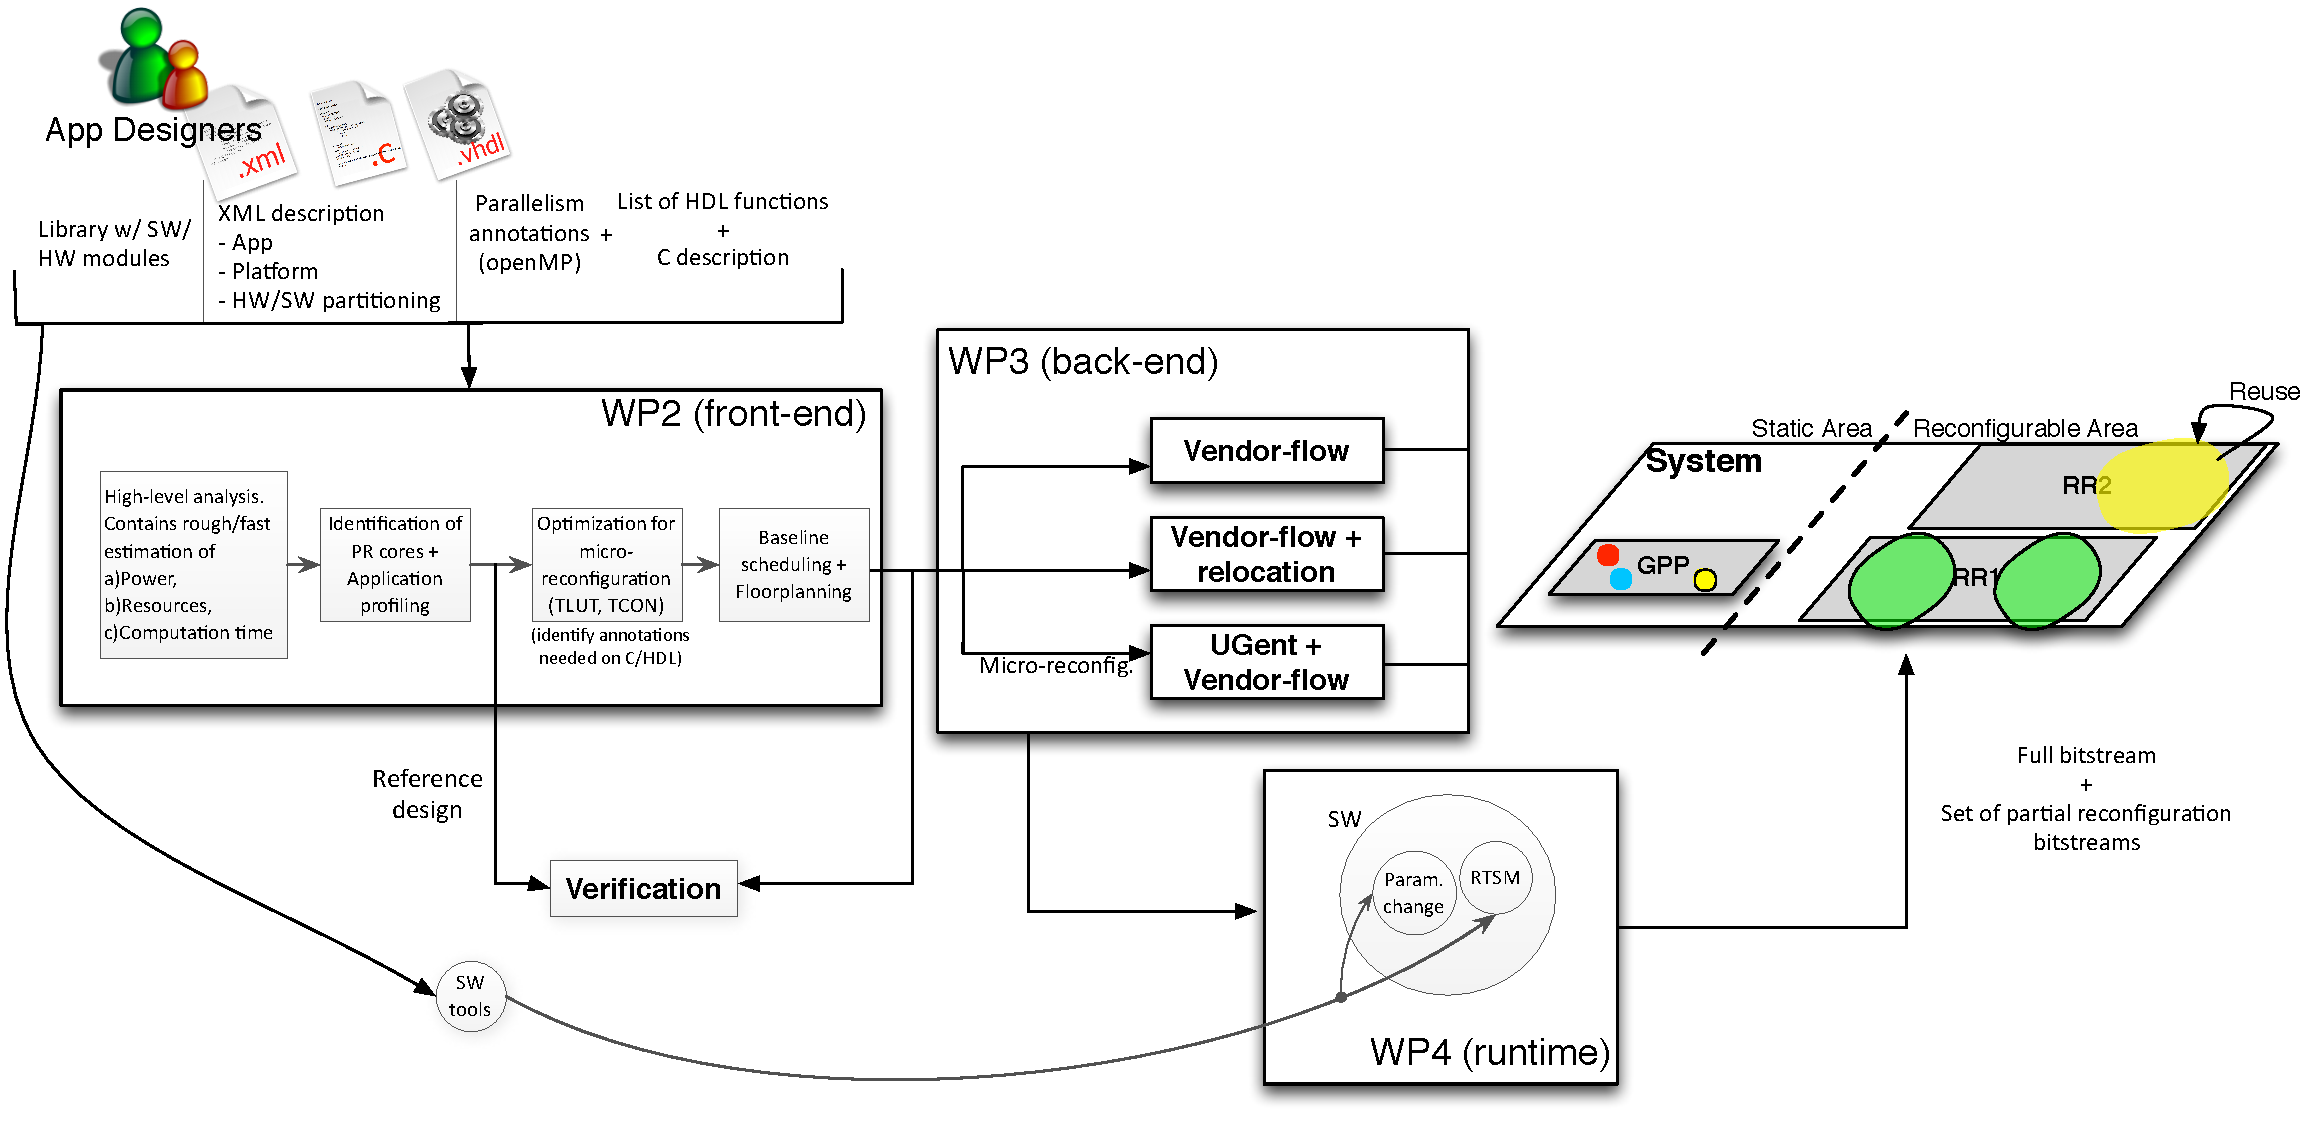
\includegraphics[width=0.9\textwidth]
{capitoli/figure/cap2/FASTERWorkflow.pdf}
\caption{Workflow di \ac{FASTER}.}
\label{fig:FASTERWorkflow}
 \end{center}
\end{figure}

La Figura \ref{fig:FASTERWorkflow} illustra la panoramica della metodologia 
adottata da \ac{FASTER} e il flusso di lavoro che, partendo dalla specifica 
dell'applicazione annotata e dalla descrizione dell'architettura target, riesce 
a derivare un bitfile utilizzabile per configurare l'architettura ed eseguire 
l'applicazione tramite un runtime manager.

L'approccio adottato da \ac{FASTER} prevede che i vari componenti del framework 
si interfaccino tra loro mediante l'uso di file XML. L'input di un progetto 
\ac{FASTER} è costituito dall'applicazione da sintetizzare, che può 
essere scritta in un linguaggio ad alto livello (ad esempio, il linguaggio C) e 
provvista di annotazioni, ad esempio in formato OpenMP\footnote{OpenMP è un 
formato standard per la specifica di applicazioni parallele, che permette di 
specificare quali funzioni di un'applicazione sono parallelizzabili e di 
suddividere l'applicazione nei vari task.}, che ne consentono la suddivisione 
iniziale in task e dalla descrizione delle funzionalità di riconfigurazione a 
disposizione dell'architettura. Oltre all'applicazione possono essere presenti 
degli attributi specificati dal designer che impongono vincoli particolari 
all'applicazione, quali ad esempio scadenze nell'esecuzione oppure una 
richiesta in termini di throughput.

\paragraph{High-level analysis}
La prima fase del flusso di lavoro prevede l'analisi ad alto livello 
dell'applicazione e dei suoi requisiti. In questa fase è fornito un modello di 
design riconfigurabile che mette in relazione i requisiti dell'applicazione con 
determinate metriche di valutazione delle performance.

Tramite questo processo si possono identificare dei componenti e determinare le 
performance delle relative implementazioni: esempi di parametri relativi ad 
un'implementazione sono le stime di risorse occupate, dell'overhead introdotto 
dalle riconfigurazioni o del consumo di energia in base all'area occupata su 
scheda.

\paragraph{Identificazione dei core}
Durante questa fase viene analizzata l'applicazione per estrarne i vari core, 
ovvero moduli composti da una serie di operazioni. I moduli sono estratti 
partendo dal \ac{CDFG} dell'applicazione, cercando di identificare opportuni 
sottografi isomorfi; nel caso l'identificazione abbia successo, è possibile 
riutilizzare uno o più moduli senza fare uso di riconfigurazione e guadagnando 
quindi in termini di tempo di esecuzione.
I core possono essere di due tipi:
\begin{enumerate}
 \item \emph{statici}, moduli configurati staticamente e non riconfigurabili 
durante l'esecuzione;
 \item \emph{riconfigurabili}, i quali a loro volta si dividono in:
  \begin{itemize}
   \item \emph{region-based}, in cui l'intero modulo viene riconfigurato;
   \item \emph{micro-riconfigurabili}, in cui solo piccole parti del modulo 
sono riconfigurate e il resto viene riutilizzato.
  \end{itemize}
\end{enumerate}

Al termine dell'identificazione dei core, si svolge la fase di 
\emph{partitioning}, in cui si stabilisce quali parti dell'applicazione debbano 
essere eseguite in software su un processore general-purpose e quali in 
hardware su logica riconfigurabile.

\paragraph{Baseline scheduling}
A questo punto, partendo dalle informazioni calcolate nei passi precedenti, 
viene calcolato un baseline schedule dei task sulla piattaforma target. Lo 
schedule viene calcolato da uno scheduler euristico che deve essere conscio 
delle riconfigurazioni che vengono introdotte. Lo scheduler deve quindi 
avere le seguenti funzionalità:
\begin{itemize}
 \item \emph{configuration prefetching}: una riconfigurazione per un 
modulo viene eseguita il prima possibile rispetto all'inizio dell'esecuzione 
del modulo, così facendo in alcuni casi è possibile mascherare l'overhead di 
riconfigurazione;
 \item \emph{riutilizzo dei moduli}: eventuali moduli che devono 
essere eseguiti in hardware (stabilito nella fase di partitioning) e sono 
caratterizzati dalla stessa implementazione non necessitano di riconfigurazione 
dell'area.
\end{itemize}
Obiettivo di questa fase è ottenere uno scheduling \emph{feasible} che abbia il 
minore makespan possibile, non necessariamente il minimo assoluto.

Il floorplanner viene eseguito in questa fase e si occupa del piazzamento dei 
moduli sull'area della scheda \ac{FPGA}; vengono definiti i vincoli spaziali e 
la dimensione delle aree su cui configurare i moduli da eseguire, e viene 
stabilito se un determinato piazzamento è fattibile oppure viola alcuni vincoli.

\paragraph{Generazione del codice} % TODO sistemare e ampliare
In questa fase viene generato il codice necessario per eseguire l'applicazione 
sulla piattaforma target, tramite l'utilizzo di backend specifici per ogni tipo 
di piattaforma supportata.

Partendo dal progetto \ac{FASTER} così creato si può derivare un progetto 
interfacciato con i vari tool sviluppati dal fornitore della piattaforma target 
per la sintesi dei vari IP core o del sistema di comunicazione tra i moduli.


\subsubsection{Conclusioni}
In questa sezione si è fornita una descrizione del progetto europeo 
\ac{FASTER}. Sono state descritte le motivazioni e il fondamento logico alla 
base del progetto, gli obiettivi che esso si profigge di raggiungere nel 
facilitare il design di applicazioni per dispositivi in grado di sfruttare le 
potenzialità offerte dalla \emph{riconfigurazione}. Infine, è stato esaminato 
ad alto livello il flusso di lavoro del progetto e le varie fasi in cui questo 
si divide sono state descritte brevemente.

Nella prossima sezione ci si concentrerà sul lavoro oggetto di questa tesi, 
ovvero la fase di baseline scheduling del progetto; verranno presentate alcune 
soluzioni presenti nello stato dell'arte riguardanti questo problema, con 
relativi pregi e difetti di ognuna.


\section{Algoritmi proposti}
\label{sec:algoritmiProposti}
In questa sezione verranno esaminate diverse soluzioni al problema dello 
scheduling, proposte in altri lavori.

Come anticipato nel Capitolo \ref{chap:intro}, il problema di trovare uno 
schedule di lunghezza minima per un insieme di task in presenza di vincoli di 
risorse appartiene alla classe dei problemi di ottimizzazione 
$\mathcal{NP}$-difficili. Tutte le soluzioni proposte appartengono a una 
tra queste categorie di algoritmi:
\begin{enumerate}
 \item \emph{algoritmi esatti} o \emph{ottimi}, che permettono di ricavare la 
soluzione ottima, tramite l'impiego di opportune strutture matematiche o di 
formulazioni particolari del problema;
 \item \emph{algoritmi euristici}, che in generale portano ad ottenere 
soluzioni subottime. Gli algoritmi euristici si possono suddividere a loro 
volta in sottocategorie in base al loro funzionamento, tra le più importanti 
ricordiamo:
 \begin{itemize}
  \item euristiche basate su una lista, in cui i task vengono schedulati 
secondo l'ordine in cui compaiono nella lista ordinata per priorità decrescenti;
  \item meta-euristiche, che comprendono algoritmi evolutivi o ispirati al 
comportamento di sistemi presenti in natura.
 \end{itemize}
\end{enumerate}

\begin{figure}
 \begin{center}
  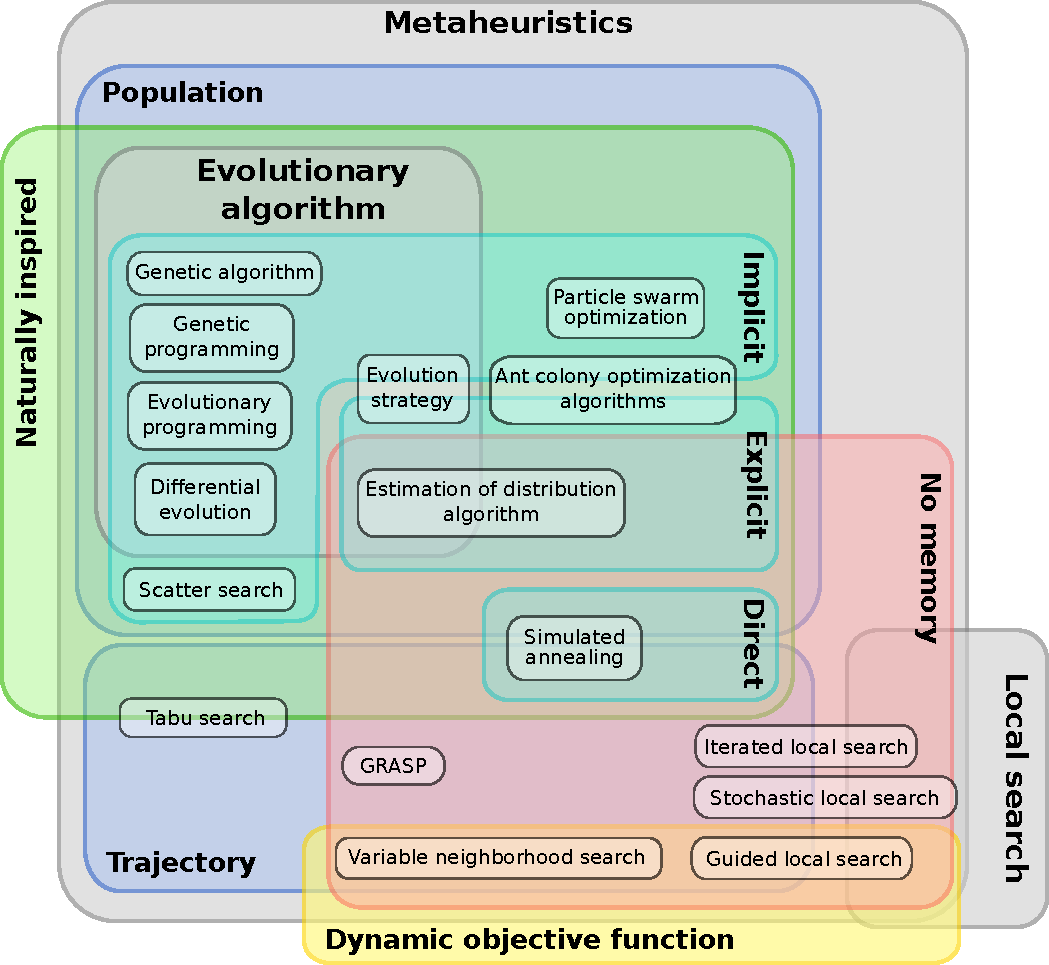
\includegraphics[width=0.7\textwidth]
  {capitoli/figure/cap2/MetaheuristicsClassification.pdf}
  \caption{Classificazione delle varie categorie di meta-euristiche. Immagine 
realizzata da Johann Dréo e tradotta in inglese da Caner Candan.}
\label{fig:metaheuristicsClassification}
 \end{center}
\end{figure}

%%%%%%%%%%
\acrodef{SCOP}{Stochastic Combinatorial Optimization Problem}
%%%%%%%%%%

La classificazione dei diversi tipi di algoritmi meta-euristici è illustrata in 
Figura \ref{fig:metaheuristicsClassification}. Diversi lavori forniscono 
un'analisi di questo tipo di algoritmi euristici, ad esempio lo studio condotto 
da Bianchi et al. \cite{SurveyMetaheuristicSCOP} analizza l'impiego delle 
meta-euristiche per la risoluzione di \acp{SCOP} o l'analisi effettuata da Blum 
et al. \cite{MetaheuristicCombinatorialOptimization} per problemi di 
ottimizzazione combinatoria.

Il resto della sezione è organizzato come segue: nella Sezione 
\ref{sec:algoritmiEsatti} vengono descritte le soluzioni proposte per il 
problema dello scheduling basate su algoritmi esatti; la Sezione 
\ref{sec:algoritmiEuristici} presenta invece le soluzioni basate su metodi 
euristici.


\subsection{Algoritmi esatti}
\label{sec:algoritmiEsatti}
Come esposto nell'introduzione a questa sezione, gli algoritmi esatti 
permettono di ottenere la soluzione ottima in assoluto. Un algoritmo esatto, 
applicato a un problema di ottimizzazione combinatoria qual è un \ac{RCSP}, 
permette di ottenere lo schedule caratterizzato dal minimo makespan possibile. 

A prescindere dal particolare algoritmo utilizzato per risolvere il problema, 
il costo computazionale necessario per giungere a una soluzione è elevato e 
solitamente non polinomiale, a meno di istanze del problema molto particolari e 
in generale difficilmente riscontrabili in casi reali 
\cite{PolynomialCompleteScheduling}.

Nelle prossime sezioni verranno esaminate alcune soluzioni proposte per 
ottenere una soluzione ottima al problema oggetto del lavoro.

\subsubsection{Programmazione lineare}
La programmazione lineare, in inglese \ac{LP}, è un metodo matematico che, 
applicato a un modello con requisiti sotto forma di vincoli \emph{lineari}, 
permette di ricavare la soluzione ottima tra tutte le soluzioni possibili che 
soddisfano i requisiti. L'ottimità della soluzione è determinata in base a una 
funzione (lineare) detta \emph{funzione obiettivo}.

Il problema è tradotto matematicamente nei termini di un modello, 
caratterizzato da \emph{variabili}, \emph{parametri} e \emph{vincoli}.
La \emph{forma canonica} di un problema di programmazione lineare è espressa 
come:

\begin{align*}
& \text{maximize}   && \mathbf{c}^\mathrm{T} \mathbf{x}\\
& \text{subject to} && A \mathbf{x} \le \mathbf{b},\\
&  && \mathbf{x} \ge \mathbf{0}
\end{align*}

Alternativamente, si può esprimere in maniera equivalente utilizzando la 
\emph{forma standard}:

\begin{align*}
 & \text{maximize}   && \mathbf{c}^\mathrm{T} \mathbf{x}\\
& \text{subject to} && A \mathbf{x} = \mathbf{b}, \\
&  && \mathbf{x} \ge \mathbf{0}
\end{align*}
dove $\mathbf{x}$ rappresenta il vettore di variabili che devono essere 
determinate per trovare la soluzione ottima, $\mathbf{c}$ e $\mathbf{b}$ sono 
vettori di coefficienti costanti e noti, $\mathbf{A}$ è una matrice di 
coefficienti e $(\mathord{\cdot})^\mathrm{T}$ 
rappresenta la trasposizione della matrice/vettore.

È sempre possibile passare dalla forma canonica alla forma standard 
introducendo variabili aggiuntive, dette variabili di \emph{scarto}, che 
permettono di eliminare le disequazioni nei vincoli; le variabili del problema 
che non presentano vincoli di segno possono essere sostituite dalla differenza 
tra due variabili aventi vincoli di segno.

Un problema di programmazione lineare intera, a differenza da un problema di 
programmazione lineare (come mostrato nelle precedenti forme), aggiunge un 
vincolo di interezza per le variabili decisionali contenute nel vettore 
$\mathbf{x}$; inoltre, i coefficienti dei vettori $\mathbf{c}$ e $\mathbf{b}$ 
e della matrice $\mathbf{A}$ sono numeri interi.

I vincoli di interezza possono anche riguardare soltanto alcune variabili o 
coefficienti, in tal caso si parla di problemi \ac{MILP}.

Nel caso dello scheduling di un grafo di task, le formulazioni proposte nello 
stato dell'arte presentano modelli con vincoli di interezza per tutte le 
variabili e i coefficienti, sono quindi problemi di programmazione lineare 
intera; i lavori di questo tipo sono descritti nella sezione seguente.


\subsubsection{Formulazioni \acs{ILP}}
Il problema di effettuare lo scheduling di task di un'applicazione per 
l'esecuzione su hardware, anche riconfigurabile, è un tema ampiamente discusso 
in letteratura; molte sono le formulazioni che ricorrono alla programmazione 
lineare intera per trovare una soluzione a questo problema. Spesso, oltre alla 
ricerca di una soluzione per lo scheduling, il modello consente anche di 
determinare un mapping adeguato che minimizzi il tempo di esecuzione finale
dell'applicazione.

Come visto nel Capitolo \ref{chap:intro}, infatti, la minimizzazione assoluta 
del tempo di esecuzione può essere ottenuta solamente risolvendo unitamente le 
fasi di mapping, scheduling e floorplanning (per verificare che la soluzione 
sia implementabile). In generale, la risoluzione separata delle fasi, in 
particolare la separazione di mapping e scheduling, non porta alla 
minimizzazione assoluta del tempo di esecuzione. La scelta tra queste due 
possibilità implica il dover fare un compromesso tra l'accuratezza della 
soluzione, che può non essere la migliore se i problemi sono risolti 
separatamente, e la dimensione dello spazio delle soluzioni possibili, che 
cresce nel caso in cui i problemi si risolvano congiuntamente.

\paragraph{Modello \acs{ILP} di Banerjee}
\label{par:BanerjeeILP}
Banerjee et al.~\cite{BanerjeePhysicalConstraints} propongono, nel loro 
articolo, un modello \ac{ILP} che prende in considerazione una 
tecnica utilizzata anche in un altro loro lavoro 
\cite{BanerjeeReconfigurationOverhead}nell'ambito delle architetture 
riconfigurabili per ridurre il tempo di esecuzione, dato il considerevole 
overhead introdotto dalle riconfigurazioni che devono essere eseguite: il 
\emph{configuration prefetching}. Per ridurre il significativo overhead delle 
riconfigurazioni, il configuration prefetching scompone un task nelle componenti 
di riconfigurazione e di esecuzione. In questo modo si permette al componente 
relativo alla riconfigurazione di essere eseguito separatamente dal task di 
esecuzione che segue, eliminando le dipendenze dai dati rappresentate dagli 
archi entranti nel task orginale.

\subparagraph{Vincoli di risorse hardware e comunicazioni}
Nello stesso lavoro \cite{BanerjeePhysicalConstraints}, Banerjee et al.~tengono 
in considerazione i vincoli di piazzamento dei task per verificare che la 
soluzione sia esatta e implementabile: infatti, tutti i task selezionati per 
l'esecuzione su scheda nella fase di partizionamento devono essere 
posizionabili senza violare la disponibilità delle risorse o le possibilità del 
controllore di riconfigurazione.

\begin{figure}[!htb]
 \begin{center}
  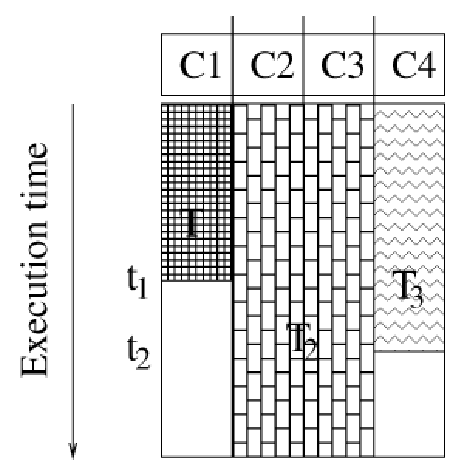
\includegraphics[width=0.3\textwidth]
{./capitoli/figure/cap2/InfeasiblePlacement.pdf}
\caption[Piazzamento ottimo non implementabile]{Esempio di piazzamento ottimo 
ma non implementabile\footnotemark.}
\label{fig:infeasiblePlacement}
 \end{center}
\end{figure}

\footnotetext{Immagine tratta da 
\cite{BanerjeePhysicalConstraints}.}

Un esempio di piazzamento di una soluzione ricavata tramite un algoritmo esatto 
per il partizionamento e lo scheduling di task nel caso di 
architettura con riconfigurazione monodimensionale è rappresentato in 
Figura \ref{fig:infeasiblePlacement}. Si ipotizzi che i requisiti di area per i 
task $T_1$, $T_2$ e $T_3$ siano $1$, $2$, e $1$ colonne, rispettivamente, e che 
sia dato il seguente mapping: $\langle T_1, C_1 \rangle$, $\langle T_2, \{C_2, 
C_3\} \rangle$ e $\langle T_3, C_4 \rangle$. Dovendo piazzare un nuovo task 
$T_4$, il cui requisito di area è pari a due colonne, un algoritmo che non 
considera le posizioni in cui vengono piazzati i vari task, vedrebbe che al 
tempo $t_2$ vi sono due colonne libere; tuttavia, non essendo colonne 
adiacenti, il piazzamento non è possibile. Da questa situazione si evince che 
la fattibilità del piazzamento lineare non è garantita dall'utilizzo di un 
algoritmo esatto.

\subparagraph{Modello e vincoli}
Il modello \ac{ILP} proposto nel loro lavoro prevede quindi la presenza di $n$ 
task che possono avere più implementazioni possibili, sia di tipo SW che HW. 
Nel caso delle implementazioni di tipo HW, ciascuna di esse ha un proprio 
requisito in termini di numero di colonne richieste\footnote{Ricordiamo che 
poichè l'architettura supporta la riconfigurazione solamente a una dimensione, 
è sufficiente specificare il numero di colonne necessarie per 
un'implementazione.}. I vincoli di risorse sono modellizzati considerando un 
processore per l'esecuzione di task SW e fissando un parametro $m$ che 
rappresenta il vincolo sul numero di colonne per il mapping dei task con 
implementazione di tipo HW.

Il configuration prefetching è modellizzato invece creando due variabili 
diverse per ogni task (se la sua implementazione è di tipo HW):
\begin{itemize}
 \item una variabile che rappresenta l'inizio della riconfigurazione;
 \item una variabile che rappresenta l'inizio dell'esecuzione.
\end{itemize}
Per tenere in considerazione i vincoli sulle risorse disponibili e sul 
piazzamento, le variabili che coinvolgono i task mappati su hardware sono 
caratterizzate, oltre a un indice che specifica il task e uno che definisce 
l'istante di tempo, da un indice aggiuntivo che rappresenta la colonna più a 
sinistra del loro mapping. In questo modo è possibile definire vincoli che 
prevengano la sovrapposizione di aree assegnate a task diversi e che rispettino 
in ogni istante la disponibilità di risorse.

\subparagraph{Limitazioni}
La principale limitazione del lavoro proposto in 
\cite{BanerjeePhysicalConstraints} è costituita dal fatto che il modello è 
adatto solo ad architetture che supportano la riconfigurazione parziale a una 
dimensione con un singolo controllore di riconfigurazione, un tipo di 
architettura molto semplice rispetto ai dispositivi utilizzabili oggigiorno. 
Inoltre, non sono considerate alcune caratteristiche sfruttabili grazie ai 
dispositivi aventi riconfigurazione parziale dinamica, ovvero il \emph{riuso 
dei moduli} ed eventuali tecniche per evitare un'eccessiva \emph{frammentazione} 
delle aree occupate dai task sulla scheda.


\paragraph{Modelli \acs{ILP} di Redaelli}
La formulazione \ac{ILP} proposta da Redaelli et al.~\cite{Redaelli1DILP} cerca 
di superare alcune limitazioni che caratterizzano i lavori 
\cite{BanerjeeHwSwPartitioning} e \cite{BanerjeePhysicalConstraints} visti nel 
precedente paragrafo. % FIXME
Il modello proposto consente infatti di tenere conto delle due tecniche 
sopracitate:
\begin{itemize}
 \item riutilizzo dei moduli, che permette a task diversi che hanno la stessa 
implementazione di essere eseguiti sulla stessa area della scheda (che quindi, 
deve essere configurata soltanto una volta invece che due);
 \item tecniche di anti-frammentazione, che permettono di ridurre la 
frammentazione dello spazio disponibile sulla scheda, così da massimizzare la 
dimensione di aree libere (adiacenti).
\end{itemize}

\subparagraph{Modello \acs{ILP} per architetture riconfigurabili a una 
dimensione}
Il primo modello proposto da Redaelli et al.~in \cite{Redaelli1DILP} è simile 
al modello formulato in \cite{BanerjeePhysicalConstraints}, ma è esteso con 
variabili e costanti che permettono di definire il concetto di riutilizzo dei 
moduli, visto in precedenza. In particolare, è definita una costante 
binaria $a_{ij}$, che assume valore $1$ se i task $i$ e $j$ eseguono la stessa 
azione (quindi il modulo è riutilizzabile); nel modello è inoltre presente una 
variabile binaria $m_i$ che assume valore $1$ se il task $i$ sfrutta un modulo 
riutilizzabile.

I vincoli a cui è soggetto il modello sono formulati in modo da evitare la 
definizione dell'istante iniziale della riconfigurazione di particolari task, 
nel caso in cui tali task sfruttino dei moduli riutilizzabili.

\subparagraph{Modello \acs{ILP} per architetture riconfigurabili a due 
dimensioni}
Il modello proposto da in \cite{Redaelli1DILP} risolve la limitazione 
riguardante la mancata considerazione della possibilità di riutilizzare alcuni 
moduli per guadagnare in termini di overhead di riconfigurazione, ma rimane un 
modello applicabile ad architetture piuttosto datate, dato che supporta 
solamente la riconfigurazione a una dimensione. Per questo, Redaelli et al.~in 
\cite{Redaelli2DILP} propongono una formulazione \ac{ILP} adatta ad 
architetture con riconfigurazione parziale dinamica a due dimensioni.

% TODO spiegare vantaggi riconfigurazione bidimensionale, qui o 
% nell'introduzione

Il modello è ripreso dal loro lavoro precedente \cite{Redaelli1DILP}, ma 
subisce alcune modifiche atte a supportare la bidimensionalità della 
riconfigurazione e delle aree da piazzare sul dispositivo.

\subparagraph{Descrizione del problema}
In primo luogo, a differenza del precedente lavoro dello stesso autore e 
del lavoro di Banerjee, cambia la descrizione del problema riguardo alla 
modellazione del dispositivo riconfigurabile. Esso non è più rappresentato 
solamente tramite un insieme di colonne $C = \{c_1,c_2,\dots,c_{\vert C 
\vert}\}$, ma anche tramite un insieme $R = \{r_1,r_2,\dots,r_{\vert R \vert}\}$ 
che ne definisce le righe. Ogni ``cella'' della \ac{FPGA} è quindi identificata 
da una coppia $(r,c)$ con $r \in R$ e $c \in C$, ed è composta da $\rho_u$ 
\acp{CLB}.

\subparagraph{Supporto alla riconfigurazione bidimensionale}
Alcune variabili del modello \ac{ILP} proposte in \cite{Redaelli1DILP} sono 
adattate per supportare la bidimensionalità dell'architettura; gli indici che 
identificano la posizione di un task (o l'occupazione temporale di una certa 
area della scheda) sono quindi due, uno per la colonna più a sinistra e uno per 
la riga più in basso.


\paragraph{Limitazioni formulazioni \acs{ILP}}
Oltre alla limitazione dovuta alle potenzialità dell'architettura 
riconfigurabile considerata in \cite{BanerjeePhysicalConstraints}, esiste uno 
svantaggio specifico per le formulazioni di programmazione lineare intera: il 
costo computazionale eccessivo. Al crescere della complessità del modello, il 
costo in termini di tempo d'esecuzione del \emph{solver \ac{ILP}} aumenta 
esponenzialmente.

Come riportato in \cite{Redaelli2DILP}, il tempo impiegato per risolvere in 
maniera ottima un'istanza del problema con $10$ task da mappare su una 
\ac{FPGA} con $5$ righe, $5$ colonne e $2$ controllori di riconfigurazione è di 
$39$ giorni, troppo per essere applicabile ad esempi concreti.


\subsubsection{Altri algoritmi ottimi}
% FIXME meglio metterne anche altri, se ci sono...
In questa sezione viene descritto un algoritmo proposto per risolvere in 
maniera ottima il problema di scheduling dei task su dispositivi 
riconfigurabili dinamicamente, che non rientra tra le formulazioni di 
programmazione lineare (intera). L'algoritmo, presentato da Fekete, K\"ohler 
e Teich in \cite{FeketeOptimal}, permette di risolvere due tipi di problemi 
legati allo scheduling:
\begin{enumerate}
 \item trovare il tempo di esecuzione minimo di un problema data una \ac{FPGA} 
con un limite di risorse fissato;
 \item trovare il numero di risorse minimo di cui deve disporre una \ac{FPGA} 
affinchè il tempo di esecuzione sia inferiore a un limite massimo fissato.
\end{enumerate}

Questo lavoro è stato il primo a comprendere la modellazione delle 
comunicazioni tra i vari moduli, includendo il ritardo dovuto alle 
comunicazioni nel tempo di esecuzione dei task.

\begin{figure}[!tb]
 \begin{center}
  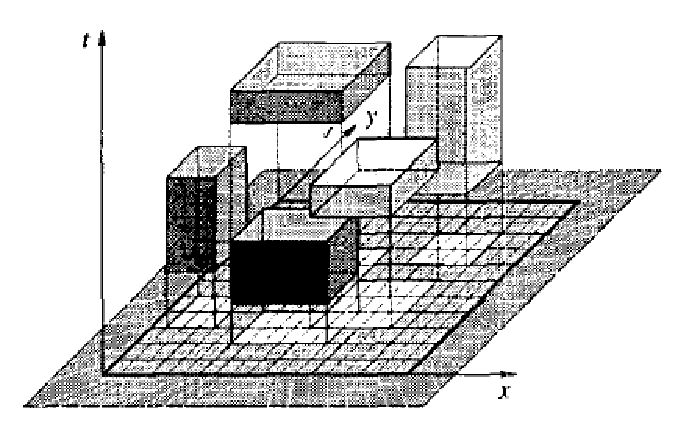
\includegraphics[width=0.5\textwidth]
{capitoli/figure/cap2/BoxModules.pdf}
\caption[Piazzamento dei moduli con rappresentazione tridimensionale]{Esempio 
di piazzamento dei moduli con rappresentazione tridimensionale\footnotemark.}
\label{fig:boxModules}
 \end{center}
\end{figure}

\footnotetext{Immagine tratta da \cite{FeketeOptimal}.}

\paragraph{Modello matematico}
I moduli sono rappresentati nel modello come box di forma tridimensionale, come 
mostrato in Figura \ref{fig:boxModules}. Nella rappresentazione utilizzata, gli 
assi $x$ e $y$ identificano le due dimensioni spaziali (per il piazzamento del 
modulo sulla scheda), mentre l'asse $t$ identifica la dimensione temporale 
(ovvero il tempo di esecuzione). È importante quindi che i moduli vengano 
piazzati dentro all'area disponibile e non si sovrappongano se eseguiti 
simultaneamente.

L'idea alla base del metodo è di trattare i task come scatole tridimensionali e 
i possibili schedule \emph{feasible} come disposizioni di tali scatole che 
soddisfano i vincoli di precedenza.

\paragraph{Limitazioni}
La principale limitazione del modello proposto in \cite{FeketeOptimal} è 
l'assunzione che ci sia un numero potenzialmente infinito di controllori di 
riconfigurazione, un'ipotesi che toglie realismo nell'applicazione del metodo 
in scenari concreti; infatti, l'overhead introdotto dalle riconfigurazioni non 
è trascurabile e l'esecuzione di un numero considerevole di riconfigurazioni 
diventa inevitabilmente un collo di bottiglia, penalizzando il tempo di 
esecuzione.


\subsection{Algoritmi euristici}
\label{sec:algoritmiEuristici}
Dopo aver fornito una panoramica degli algoritmi esatti vengono ora esaminate 
alcune soluzioni euristiche presenti nello stato dell'arte. In generale, le 
soluzioni prodotte da algoritmi euristici per un problema non sono ottime 
(esatte). Si ricorre all'impiego di algoritmi euristici qualora altri metodi 
esatti non possono essere applicati oppure sono troppo lenti nel risolvere il 
problema; in questi casi, si deve sempre trovare un compromesso tra la 
``bontà'' della soluzione trovata e il tempo impiegato per giungere a quella 
soluzione.

Le euristiche si classificano in base al modo di trovare una soluzione 
approssimata.
%%%%%%%%%%%%% FIXME controllare
Uno stesso problema può essere risolto utilizzando più di una 
euristica, ma non è garantito che tutte le euristiche applicate a uno stesso 
problema restituiscano la stessa soluzione.

Esistono euristiche specifiche per risolvere determinate classi di problemi che 
si distinguono in base al grado di approssimazione delle soluzioni trovate. 
In tal senso, un'euristica potrebbe performare meglio di altre, se applicata 
allo stesso problema.
%%%%%%%%%%%%%

\subsubsection{Partizionamento HW-SW}
Tra l'ampia varietà di algoritmi euristici proposti nello stato dell'arte per 
risolvere il problema di scheduling dei task, alcuni di questi algoritmi 
considerano come ulteriore obiettivo il partizionamento tra task hardware e 
task software. Ad esempio, Mei et al.~propongono in 
\cite{MeiPartitioningScheduling} un approccio basato sulla combinazione di un 
algoritmo genetico standard\footnote{Gli algoritmi genetici appartengono alle 
meta-euristiche di tipo evolutivo ispirate al funzionamento di sistemi presenti 
in natura, come rappresentato in Figura 
\ref{fig:metaheuristicsClassification}.} con un'euristica basata su lista di 
priorità. Il loro metodo è adatto ad architetture riconfigurabili dinamicamente 
e risolve, oltre allo scheduling, anche il partizionamento dei task che 
compongono l'applicazione.

Per la fase di partizionamento, nella quale viene deciso il tipo 
di implementazione da utilizzare per ogni task (software o hardware), si usa un 
algoritmo genetico che al suo interno esegue lo scheduling come subroutine per 
effettuare la valutazione di una determinata partizione.

L'overhead introdotto dalla riconfigurazione parziale è tenuto in 
considerazione e aggiunto al tempo di computazione dei task; tuttavia, non 
vengono impiegate tecniche per mascherare il tempo di riconfigurazione (come il 
\emph{configuration prefetching}), e il collo di bottiglia causato dalle 
limitazioni del controllore della riconfigurazione, che impongono 
riconfigurazioni non sovrapposte nel tempo.


\subsubsection{\acl{EPR} e \acl{IR}}
Jeong et al.~propongono in \cite{JeongHWSWCosynthesis} due metodi diversi per 
risolvere problemi di \emph{hardware-software cosynthesis}: una formulazione 
\ac{ILP} per risolvere in modo esatto il problema di hardware-software 
cosynthesis e una euristica.

L'algoritmo euristico si basa sull'euristica iterativa proposta da 
Fiduccia-Mattheyses in \cite{FiducciaMattheyses} per risolvere il problema del 
bipartizionamento di un ipergrafo.

In entrambi i metodi (\ac{ILP} ed euristica) vengono incorporati due concetti 
nel calcolo del trade-off del partizionamento hardware-software, per meglio 
sfruttare le capacità di riconfigurazione della \ac{FPGA} obiettivo:
\begin{itemize}
 \item \ac{EPR}, rappresenta il concetto di \emph{configuration prefetching};
 \item \ac{IR}, che consente di ridurre la quantità di dati necessari per la 
riconfigurazione, ovvero la dimensione del \emph{bitstream}; partendo da task 
che condividono parzialmente i dati necessari alla loro configurazione è 
possibile configurare in maniera incrementale soltanto le porzioni dei 
moduli che differiscono tra di loro, a condizione che tra le esecuzioni non si 
verifichino riconfigurazioni dell'intera area.
\end{itemize}

\subparagraph{Limitazioni}
Nonostante le precedenti strategie adottate per ridurre l'impatto dell'overhead 
introdotto dalle riconfigurazioni, la maggior limitazione del lavoro proposto 
in \cite{JeongHWSWCosynthesis} consiste nella mancata considerazione dei 
vincoli e dei limiti fisici imposti dall'architettura target. Pertanto, le 
soluzioni trovate potrebbero non essere fisicamente implementabili, pur essendo 
ottime o sub-ottime (nel caso si usi l'euristica).

\subsubsection{Euristica di Banerjee}
Nel lavoro di Banerjee et al.~\cite{BanerjeePhysicalConstraints}, lo stesso in 
cui è presentata la formulazione \ac{ILP} vista in \ref{par:BanerjeeILP}, è 
descritto anche un metodo euristico per la risoluzione dei problemi di 
partitionamento, scheduling e piazzamento fisico dei task rispettando i vincoli 
architetturali.

L'euristica proposta in \cite{BanerjeePhysicalConstraints} cerca di porre 
rimedio alle limitazioni del metodo proposto in \cite{JeongHWSWCosynthesis} 
presentate nel paragrafo precedente, considerando il piazzamento dei moduli 
come parte integrante dell'algoritmo di partizionamento e scheduling.

\acrodef{BRAM}{Block Random Access Memory}

Il loro approccio si basa, su un'euristica iterativa, come formulata da 
Kernighan-Lin \cite{KernighanLin} e Fiduccia-Mattheyses 
\cite{FiducciaMattheyses}. Per tenere conto di possibili ottimizzazioni 
effettuate dai compilatori, è supportata l'esistenza di più di una 
implementazione per ogni task. Un'altra importante caratteristica 
dell'euristica proposta, naturale conseguenza del tenere in considerazione i 
vincoli hardware durante il piazzamento fisico dei moduli, è la possibilità di 
estendere l'approccio per supportare l'eterogeneità di 
risorse\footnote{L'eterogeneità delle risorse consiste nell'avere delle 
risorse aggiuntive incorporate sul die, ad esempio memorie a blocchi 
(\acs{BRAM}), \acp{DSP}, moltiplicatori. Ciò consente ai designer di 
utilizzare le risorse aggiuntive presenti, senza bisogno di implementare 
manualmente tutte le funzionalità necessarie. Le risorse incorporate sono 
anche chiamate processori hardcore, in contrapposizione ai processori 
softcore, che rappresentano unità computazionali implementate usando la logica 
riconfigurabile messa a disposizione dall'\ac{FPGA}}, un fattore chiave per 
l'incremento di prestazioni delle applicazioni implementate su \ac{FPGA} 
moderne.


% TODO scendere più nel dettaglio (rappresentazione cromosomi, fitness 
% function, operatori utilizzati)


% TODO presentazione delle motivazioni che hanno portato allo sviluppo di un 
% algoritmo iterativo basato su una lista e non esplorativo

% Il flusso di esecuzione della toolchain prevede l'invocazione del tool di 
% scheduling statico come componente esterno da parte dell'algoritmo di 
% esplorazione dello spazio di design del sistema, per la valutazione di una 
% particolare metrica, la stima del tempo di esecuzione totale dello schedule 
% dato un determinato mapping. Poichè la fase di mapping è implementata sotto 
% forma di un  